\documentclass[12pt]{article}
\usepackage{graphicx}
\usepackage {color}
\usepackage{pdfpages}
\usepackage{float}
\usepackage{changebar}
\usepackage{enumitem,amssymb}
\renewcommand{\familydefault}{\sfdefault}
\usepackage[margin=1.2in]{geometry}
\usepackage{graphicx}
\usepackage{wrapfig}
\usepackage[super]{cite}
\usepackage{subcaption}
\usepackage[table]{xcolor}
\usepackage{amsmath}
\usepackage[sort, numbers]{natbib}
\usepackage{multirow}
\usepackage{tabularx}

%%%%%%%%%%%%Defining the margins %%%%%%%%%%%%%%%%%%%%%
\textheight 9.in
\textwidth 6.5in
\topmargin -.5in
\oddsidemargin 0in
\setlength{\parskip}{\smallskipamount}

%%%%%%%%%%%%%%Specific Commands %%%%%%%%%%%%%%%%%%
\newcommand{\eg}{{\em e.g.,}}
\newcommand{\ie}{{\em i.e.,}}
\newcommand{\etc}{{\em etc.,}}
\newcommand{\etal}{{\em et al.}}
\newcommand{\degrees}{{$^{\circ}$}}
\newcommand{\fig}[1]{\textbf{Figure #1}}

%%%%%%%%%%%%%%%%%%%%%%%%%%%% Setting to control figure placement
% These determine the rules used to place floating objects like figures 
% They are only guides, but read the manual to see the effect of each.
\renewcommand{\topfraction}{.9}
\renewcommand{\bottomfraction}{.9}
\renewcommand{\textfraction}{.1}
\renewcommand{\familydefault}{\sfdefault} %setting the san serif font

%%%%%%%%%%%%%%%%%%%%%%%% Line spacing
% Use the following command for ``double'' spacing
%\setlength{\baselineskip}{1.2\baselineskip}
% and this one for an acceptable NIH spacing of 6lpi based on 11pt
%\setlength{\baselineskip}{.9\baselineskip}
% The baselineskip does not appear to work when we include a maketitle
% command in the main file.  Something there must set the line spacing
% If we use this next command, then things seem to work.
\renewcommand{\baselinestretch}{.9}

\setcounter{secnumdepth}{0} %make no numbers but have a table of contents


\begin{document}

\title{Lab }
\author{Jake Bergquist, u6010393}
\maketitle
\tableofcontents
\newpage

\section{Introduction}



\section{Methods}

%Setup of recording equipment

%Calibration of force sensor
\begin{figure}[H]
	\label{fig:forceCal}
	\centering
	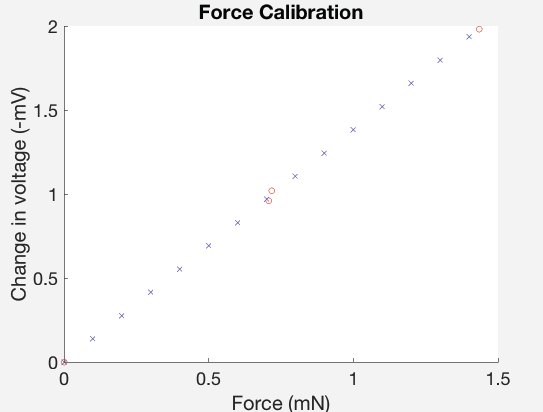
\includegraphics[width = .95\textwidth]{Figures/ForceCal.png}
	\caption{Calibration of force curve. Red circles represent measured changes in voltage for a  set of known forces (using the paperclips and gravity. The blue Xs show the fit line depicting the relationship between change in voltage and force. }
\end{figure}
%Dissection of Frog

%Frank Sterling Test

%Drug trials

%Signal processing


\section{Results}

%frank Sterling Curve

\begin{figure}[H]
	\label{fig:FSCurve}
	\centering
	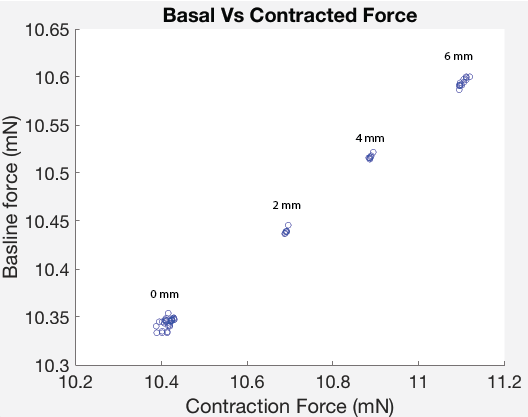
\includegraphics[width = .95\textwidth]{Figures/FSCurve.png}
	\caption{Frank Starling curve. On the x axis is contractile force and on the y axis is relaxed tension. Each cluster represents several beats at that particular stretch length from 0 mm to 6 mm. }
\end{figure}

%Baseline ecg and force curve

%Signal averaged example

\begin{figure}[H]
	\label{fig:SignalProcessing}
	\centering
	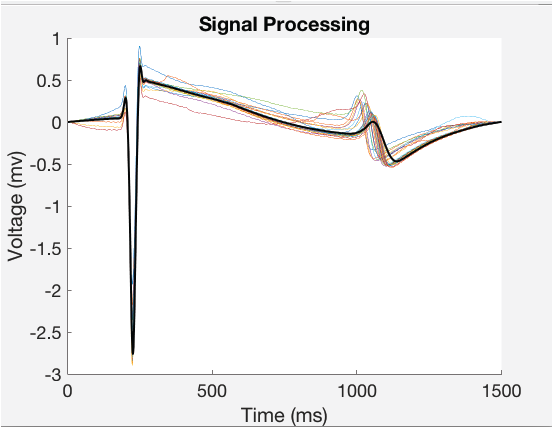
\includegraphics[width = .95\textwidth]{Figures/SP.png}
	\caption{An example fo the beat averaging. Several autofiducilized beats are shown. The beats are averaged into the signal averaged beat (black line) which has greatly reduced noise. }
\end{figure}

%Table of heart rates and contraction forces

\begin{table}[H]
	\centering
	\caption{Numerical results. Mean and Median heart rate are shown as calculated from electrode signals and force probe signals. Mean and Median contractile force is shown.}\label{tab:stats}
	%\rowcolors{2}{gray!25}{white}
	\begin{tabular}{|r r|r|r|}
		\hline
		Drug&&HR & Contraction Force \\
		\hline
		\multirow{2}{*}{Basal}
		&From Electrode & 31.61 &  \\
		&From Force Probe & 31.63 & 0.34 \\
		\hline
		\multirow{2}{*}{Cold Ringers}
		&From Electrode & 26.45&   \\
		&From Force Probe & 24.32 & 0.23 \\
		\hline
		\multirow{2}{*}{Caffeine}
		&From Electrode & 33.25&   \\
		&From Force Probe & 31.01& 0.19 \\
		\hline
		\multirow{2}{*}{Mystery Drug}
		&From Electrode & 34.12 &   \\
		&From Force Probe &33.95 & 0.18  \\
		\hline
		\multirow{2}{*}{Calcium 0.55 mM}
		&From Electrode & 35.21 & \\
		&From Force Probe & 35.04 & 0.14 \\
		\hline
		
		\multirow{2}{*}{Calcium 4.4 mM}
		&From Electrode & 31.25 &   \\
		&From Force Probe & 32.05 & 0.11  \\
		\hline
		
		\multirow{2}{*}{Epinephrine }
		&From Electrode & 33.12 &  \\
		&From Force Probe & 32.65 & 0.09 \\
		\hline
		
		\multirow{2}{*}{Acetylcholine}
		&From Electrode & 25.34 &  \\
		&From Force Probe & 26.53 & 0.02  \\
		\hline
		
		\multirow{2}{*}{Atropine}
		&From Electrode & 30.01 &   \\
		&From Force Probe & 31.25 & 0.07 \\
		\hline
		
		\multirow{2}{*}{Potassium}
		&From Electrode & 30* &   \\
		&From Force Probe & 30.41* & 0.07*  \\
		\hline
		
	\end{tabular}
\end{table}


%Drug Study:
%Force curve

\begin{figure}[H]
	\label{fig:ForceGraph}
	\centering
	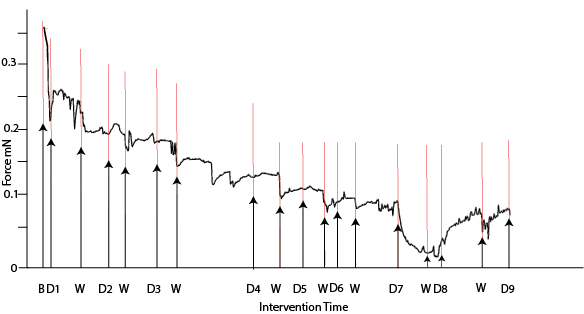
\includegraphics[width = .95\textwidth]{Figures/ForceGraph.png}
	\caption{Graph of changes in contractile force during the experiments. B represents the baseline measurement. Each W represents a time at which the heart was flushed with ringer's lactate solution to wash out. D1 was addition of Cold ringers. D2: caffeine, D3: Mystery drug, D4: 0.55 mM calcium, D5: 4.4 mM calcium. D6: Epinephrine, D7: Acetylcholine, D8: Atropine, D9: Potassium Chloride }
\end{figure}


%Baseline

\begin{figure}[H]
	\label{fig:Baseline}
	\centering
	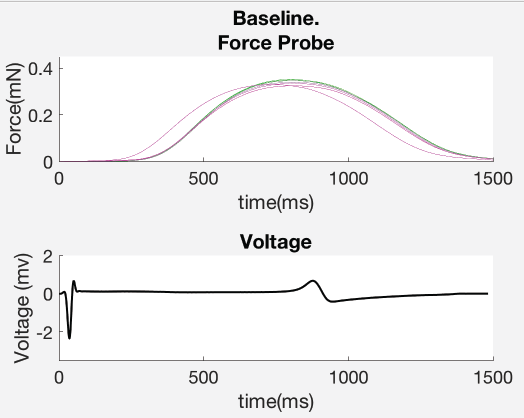
\includegraphics[width = .95\textwidth]{Figures/Baseline.png}
	\caption{Force curve and signal averaged electrical recording.(Top) Force Probe recorded force. The curves progress from green to gray to pink with time. (Bottom) Signal averaged voltage from the ventricles shown in black. }
\end{figure}

%Cold ringers

\begin{figure}[H]
	\label{fig:ColdRinger}
	\centering
	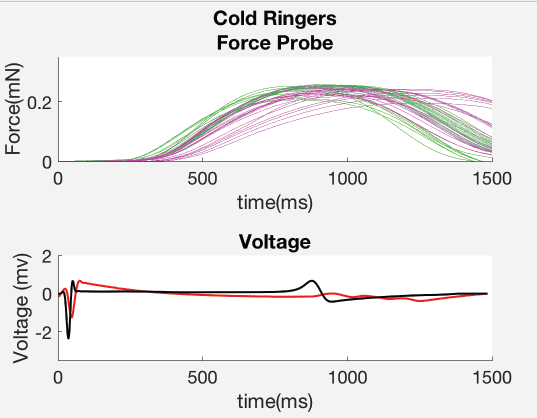
\includegraphics[width = .95\textwidth]{Figures/ColdR.png}
	\caption{Force curve and signal averaged electrical recording.(Top) Force Probe recorded force. The curves progress from green to gray to pink with time. (Bottom) Signal averaged voltage from the ventricles. Baseline signal shown in black, cold ringers signal shown in red. }
\end{figure}

%Caffine
\begin{figure}[H]
	\label{fig:Caffine}
	\centering
	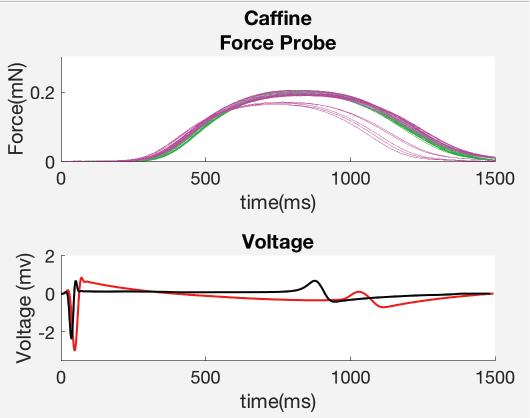
\includegraphics[width = .95\textwidth]{Figures/Caffine.png}
	\caption{Force curve and signal averaged electrical recording.(Top) Force Probe recorded force. The curves progress from green to gray to pink with time. (Bottom) Signal averaged voltage from the ventricles. Baseline signal shown in black, caffeine signal shown in red. }
\end{figure}

%Drug X
\begin{figure}[H]
	\label{fig:Drugx}
	\centering
	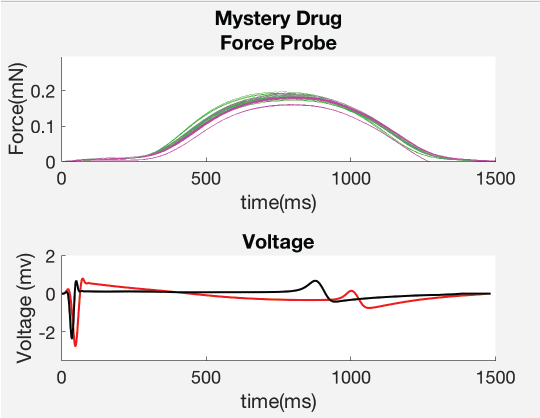
\includegraphics[width = .95\textwidth]{Figures/Drugx.png}
	\caption{Force curve and signal averaged electrical recording.(Top) Force Probe recorded force. The curves progress from green to gray to pink with time. (Bottom) Signal averaged voltage from the ventricles. Baseline signal shown in black, mystery drug signal shown in red. }
\end{figure}
%CaCl2 0.55mM
\begin{figure}[H]
	\label{fig:CalcLow}
	\centering
	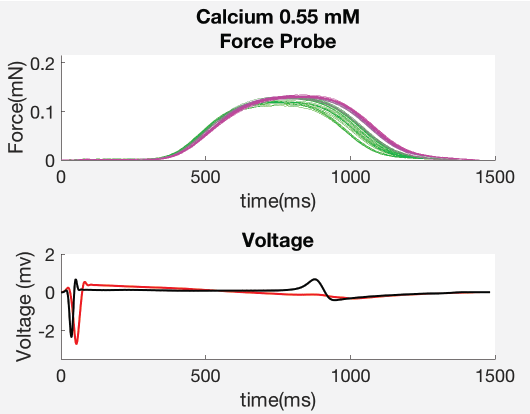
\includegraphics[width = .95\textwidth]{Figures/CalciumLow.png}
	\caption{Force curve and signal averaged electrical recording.(Top) Force Probe recorded force. The curves progress from green to gray to pink with time. (Bottom) Signal averaged voltage from the ventricles. Baseline signal shown in black, 0.55 mM Calcium signal shown in red. }
\end{figure}
%CaCl2 4.4 mM
\begin{figure}[H]
	\label{fig:CalcHigh}
	\centering
	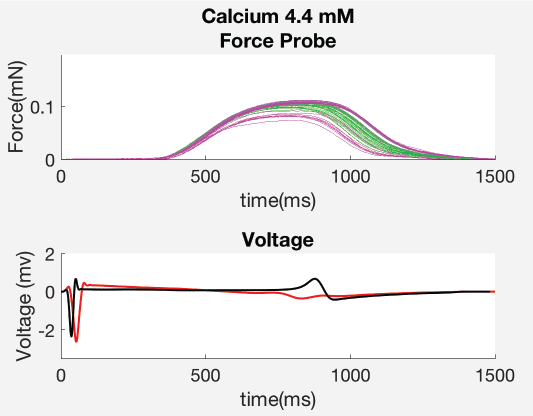
\includegraphics[width = .95\textwidth]{Figures/Calciumhigh.png}
	\caption{Force curve and signal averaged electrical recording.(Top) Force Probe recorded force. The curves progress from green to gray to pink with time. (Bottom) Signal averaged voltage from the ventricles. Baseline signal shown in black, 4.4 mM Calcium signal shown in red. }
\end{figure}
%Epi
\begin{figure}[H]
	\label{fig:Epi}
	\centering
	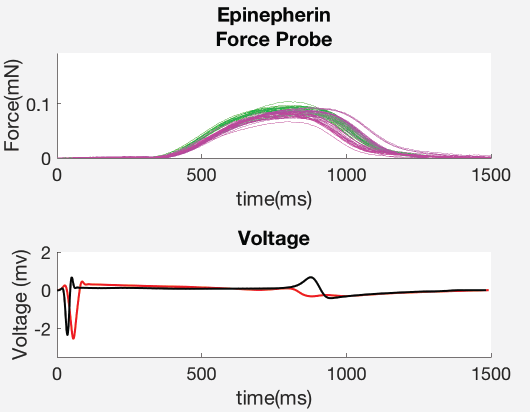
\includegraphics[width = .95\textwidth]{Figures/Epi.png}
	\caption{Force curve and signal averaged electrical recording.(Top) Force Probe recorded force. The curves progress from green to gray to pink with time. (Bottom) Signal averaged voltage from the ventricles. Baseline signal shown in black, epinephrine  signal shown in red. }
\end{figure}
%Ach 1 mM
\begin{figure}[H]
	\label{fig:Ach}
	\centering
	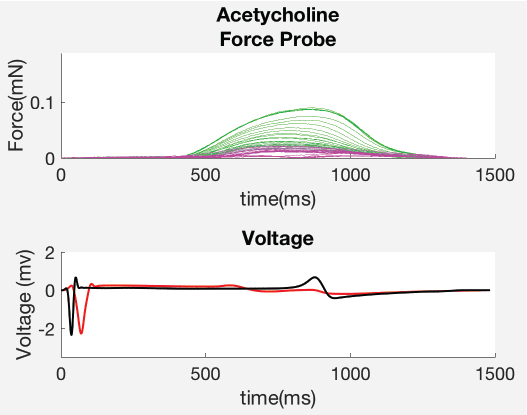
\includegraphics[width = .95\textwidth]{Figures/Ach.png}
	\caption{Force curve and signal averaged electrical recording.(Top) Force Probe recorded force. The curves progress from green to gray to pink with time. (Bottom) Signal averaged voltage from the ventricles. Baseline signal shown in black, acetylcholine signal shown in red. }
\end{figure}
%Atropine
\begin{figure}[H]
	\label{fig:Atropine}
	\centering
	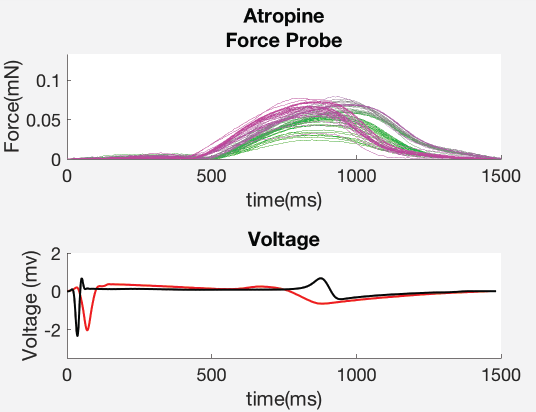
\includegraphics[width = .95\textwidth]{Figures/Atropine.png}
	\caption{Force curve and signal averaged electrical recording.(Top) Force Probe recorded force. The curves progress from green to gray to pink with time. (Bottom) Signal averaged voltage from the ventricles. Baseline signal shown in black, atropine signal shown in red. }
\end{figure}
%KCl
\begin{figure}[H]
	\label{fig:KCL}
	\centering
	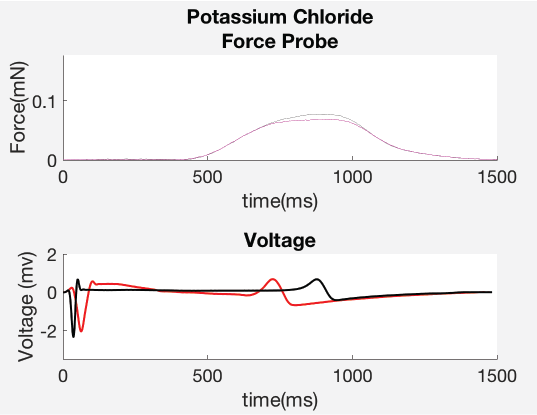
\includegraphics[width = .95\textwidth]{Figures/KCl.png}
	\caption{Force curve and signal averaged electrical recording.(Top) Force Probe recorded force. The curves progress from green to gray to pink with time. (Bottom) Signal averaged voltage from the ventricles. Baseline signal shown in black, potassium signal shown in red. }
\end{figure}
\section{Discussion}




%%%%%%%%%%%%%%%%%% Correct Bibliography Style

%\bibliography{C:/Users/Jake/Documents/library}
%\bibliographystyle{IEEEtran}


\end{document}








